\section{Queueing system}
Queueing happens in everyday life. At the supermarket or airport, bank and so on. A typical queueing system (say at the airport check-in): 


Suppose the $n^{th}$ customer $C_n$ arrives at time $\tau_n\geqslant 0$, where $\tau_n =0$ and $0\leqslant \tau_1\leqslant \tau_2\leqslant \cdots\leqslant $. The \uline{interarrival time} between customers $c_n$ and $c_{n+1}$ is $T_n = \tau_{n+1} - \tau_n\ (T_0 = \tau_1)$. The \uline{service time} for customer $C_n$ is $X_n\geqslant 0$. Assume the $T_n$ are independent random variables, and the some for the $X_n$. The \uline{distribution function (DF)} of $T_n(n\geqslant 0)$ is $A_n:\mathbb{R}\to [0, 1]$, where
\begin{align*}
    A_n(t) = \mathbb{P}(T_n\leqslant t)
\end{align*}
and the \uline{probability density function (PDF)} is 
\begin{align*}
    a_n(t) = A_n^{\prime}(t)
\end{align*}

Similarly, $X_n\ (n\geqslant 1)$ has DF $B_n(t) = \mathbb{P}(X_n\leqslant t)$ and PDF $b_n(t) = B_n^{\prime}(t)$. 

\paragraph{Kendall-Lee notation} A queueing system description is written as:

\vspace{1em}
\begin{align}
    \eqnmarkbox[red]{A}{A}/\eqnmarkbox[blue]{B}{B}/\eqnmarkbox[green]{s}{s}/\eqnmarkbox[pink]{D}{D}/\eqnmarkbox[brown]{q}{q}/\eqnmarkbox[orange]{p}{p} \label{4.1}
\end{align}
\annotate[yshift=0.5em]{above,left}{A}{Interarrival time distribution}
\annotate[yshift=2.0em]{above,left}{B}{Service time distribution}
\annotate[yshift=-0.5em]{below, left}{s}{Number of servers}
\annotate[yshift=-0.5em]{below,right}{D}{Queueing discipline}
\annotate[yshift=2.0em]{above,right}{q}{Maximum number of customers allowed in the queueing system\\ (in queue and in service)}
\annotate[yshift=0.5em]{above,right}{p}{Customer population}

\paragraph{Notable cases:}
For $A$ and $B$:
\begin{itemize}
    \item $M$: \uline{Markovian}, with \uline{exponential distribution}
    \begin{align*}
        A_n(t) = 1-e^{-\lambda_n t},\quad a_n(t) = \lambda_n e^{-\lambda_n t}
    \end{align*}
    for some parameter $\lambda_n > 0\ (n\geqslant 0)$. Similarly for $B_n(t)$, $b_n(t)$ with parameter $\mu_n>0\ (n\geqslant 1)$.
    \item $D$: \uline{Deterministic}, with ``constant distribution''.
    \item $E_k$: \uline{Erlang-k}
    \item $G$: \uline{General}, not specified, usually the mean and variance are known.
\end{itemize}

For $D$:
\begin{itemize}
    \item FCFS: \uline{First come first served}. Services is performed according to the order of the queue. New arrival join the back of the queue.
    \item LCFS: \uline{Last come first served}. 
    \item SIRO: \uline{Service in random order}.
\end{itemize}

\paragraph{Note also} Nucleic acid test queueing discipline. 

Arrival order: $1,2,\cdots, 20, 21, 22, \cdots, 40, 41, \cdots$

Service order: $20, 19, \cdots, 40, 39,\cdots, 21, 60, \cdots$

For example, $M/G/2/SIRO/50/1000$. If $D = FCFS$, $q=p=\infty$, then we write \ref{4.1} as $A/B/s$. The simplest case is $M/M/s$, especially $M/M/1$.

\begin{definition}
    
    \begin{itemize}
        \item \uline{State/Queue length}$=$ Number of customers in the queueing system/queue (12 and 8 in the diagram).
        \item $N(t) = $ State at time $t\geqslant 0$.
        \item $\mathbb{P}_k(t) = $ Probability of state $k$ at time $t\geqslant 0$ (assume $\mathbb{P}_k(0) = 0$).
        \item $\lambda_k = $ Mean arrival rate $=$ Expected number of new customer arrivals per unit time, when state $=k\geqslant 0$.
        \item $\mu_k = $ \uline{Mean service rate for overall system} $=$ Expected number of customers served per unit time between all \uline{busy} servers (those serving customers), when state $= k\geqslant 1$.
    \end{itemize}
\end{definition}

When $A$ and $B$ are both Markovian, we have the \uline{birth-death process rate diagram}:
\usetikzlibrary{automata}
\begin{tikzpicture}[->, >=stealth', auto, thick, node distance=2cm]

\tikzstyle{every state}=[fill=white, draw=black, text=black, minimum size=1.2cm]

\node[state] (q0) {$0$};
\node[state] (q1) [right of=q0] {$1$};
\node[state] (q2) [right of=q1] {$2$};
\node[state] (q3) [right of=q2] {$3$};

\path[->, draw=blue] 
    (q0) edge[bend left] node[above] {$\lambda_0$} (q1)
    (q1) edge[bend left] node[above] {$\lambda_1$} (q2)
    (q2) edge[bend left] node[above] {$\lambda_2$} (q3)
    (q3) edge[bend left] node[above] {$\lambda_3$} ($(q3)+(1,0)$);

\path[->, draw=red]
    (q1) edge[bend left] node[below] {$\mu_1$} (q0)
    (q2) edge[bend left] node[below] {$\mu_2$} (q1)
    (q3) edge[bend left] node[below] {$\mu_3$} (q2)
    ($(q3)+(1,0)$) edge[bend left] node[below] {$\mu_4$} (q3);

\end{tikzpicture}

If $\lambda_k$ is constant $\forall k\geqslant 0$, write $\lambda_k = \lambda$. If the mean service rate \uline{per busy server} is constant $\forall k\geqslant 1$, denote this constant by $\mu$. Then 
\begin{align*}
    \mu_k = \left\lbrace\begin{array}{ll}
       k_{\mu} & 1\leqslant k\leqslant s \\
        s\mu & k>s.
    \end{array} \right.
\end{align*}

Under these circumstance, $\frac{1}{\lambda}$ and $\frac{1}{\mu}$ are the \uline{expected interarrival time} and the \uline{expected service time}.

Also,
\begin{align*}
    \varrho = \frac{\lambda}{s\mu}
\end{align*}

is the \uline{utilisation factor} of the service facility, which is the expected fraction of time the service capacity $(s\mu)$ is being utilised by arriving customers $(\lambda)$.

\begin{example}
    Suppose a time unit is one hour.
    \begin{itemize}
        \item If on average, a customer arrives every 10 minutes, then $\lambda = 6$ customers/hour. Expected interarrival time $\frac{1}{\lambda} = \frac{1}{6}$.
    
        \item If on average, a service time takes 30 minutes, then $\mu = 2$ customers/hour. Expected service time $= \frac{1}{\mu} = \frac{1}{2}$.
    \end{itemize}
    Utilisation factor $\varrho = \frac{\lambda}{s\mu} = \frac{3}{s}$.
    \begin{itemize}
        \item If $s = 1,2$, then $\varrho>1$. The state $\to\infty$ as time $\to\infty$, and the system is ``unsteady''.
        \item If $s = 3$, then $\rho = 1$. Queue is unstable and system may not become ``steady''.
        \item If $s\geqslant 4$, then $\rho <1$. The system will become ``steady''. 
    \end{itemize}
\end{example}

\begin{definition}
    \begin{align}
        \eqnmarkbox[blue]{1}{\bar{L}(t)} &= \frac{1}{t}\int_0^t N(u)du \nonumber \\
        \eqnmarkbox[red]{2}{\bar{L}} &= \lim\limits_{t\to\infty} \bar{L}(t) \nonumber \\
        & {} \nonumber \\
        \eqnmarkbox[orange]{4}{\bar{\alpha}(t)} &= \frac{\eqnmarkbox[green]{3}{\alpha(t)}}{t} \nonumber \\
        \eqnmarkbox[pink]{5}{\bar{\lambda}} &= \lim\limits_{t\to\infty} \bar{\alpha(t)}  \label{4.2}
    \end{align}
    \annotate[yshift=0.5em]{above,right}{1}{The average state over $[0,t]$}
    \annotate[yshift = 0.5em]{above,left}{2}{The long term average state}
    \annotate[yshift = 0.5em]{above,right}{3}{Number of arrivals in $[0,t]$}
    \annotate[yshift = 0.5em]{above,left}{4}{The average number of arrivals in $[0,t]$}
    \annotate[yshift = -0.5em]{below,left}{5}{The long term average arrival rate}

    \begin{itemize}
        \item \uline{Sojourn time} $=$ Time a customer spends in queueing system.
        \item $W_k = $ Sojourn time of customer $C_k$.
        \item $\bar{W}(t) = \frac{1}{\alpha(t)}\sum\limits_{k=1}^{\alpha(t)} W_k$, the \uline{average sojourn time} in $[0,t]$.
        \begin{align}
            \bar{W} = \lim\limits_{t\to\infty} \frac{1}{n} \sum\limits_{k=1}^n W_k \label{4.3}
        \end{align}
        the \uline{long term average sojourn time}
    \end{itemize}
\end{definition}

\begin{theorem}[Little' Low]
    For any queueing system, 
    \begin{align}
        \overline{L} = \overline{\lambda}                                    \ \overline{W}, \label{4.4}
    \end{align}
    provided the limits \ref{4.2}, \ref{4.3} exist.
\end{theorem}
\begin{proof}
    Let $\beta(t)$ be the number of departures in $[0,t]$. We compare the graphs of $\alpha(t)$, $\beta(t)$, and the sojourn times.


    Let $E(t)$ be the excess sojourn time of all active customers beyond time $t$. Then 
    \begin{align*}
        \overline{L}(t) &= \frac{1}{t}\int_0^t N(u)du = \frac{1}{t}\int_0^t (\alpha(u) - \beta(u)) du \\
        &= \frac{\alpha}{t} \frac{1}{\alpha} \left(\sum\limits_{k=1}^{\alpha(t)}W_k - E(t) \right) = \bar{\alpha}(t) \overline{W(t)} - \frac{E(t)}{t}
    \end{align*}

    Letting $t\to\infty$ and assuming $\frac{E(t)}{t}\to 0$, \ref{4.4} follows.
\end{proof}

\begin{remark}
    If $\overline{L}(q) = $ Long term average queue length, $\overline{W}_q = $ Long term average queueing time, then we can similarly prove that
    \begin{align*}
        \overline{L}_q = \overline{\lambda}\ \overline{W}_q
    \end{align*}
    Also, if the expected service time $\frac{1}{\mu}$ is constant, then
    \begin{align*}
        \overline{W} = \overline{W}_q + \frac{1}{\mu}
    \end{align*}
\end{remark}

\begin{example}
    Bob owns a small coffee shop. He estimates that on average, in one hour, 40 customers arrive at his shop, and each customer spends 6 minutes in the queueing system. Then the average number of customers in the queueing system is 
    \begin{align*}
        \overline{L} = \eqnmarkbox[red]{1}{40}\times \eqnmarkbox[orange]{2}{0.1} = 4
    \end{align*}
    \annotate[yshift=-0.5em]{below,left}{1}{$\overline{\lambda}$}   
    \annotate[yshift=-0.5em]{below,right}{2}{$\overline{W}$}    
\end{example}

\begin{figure}[H]
    \centering
    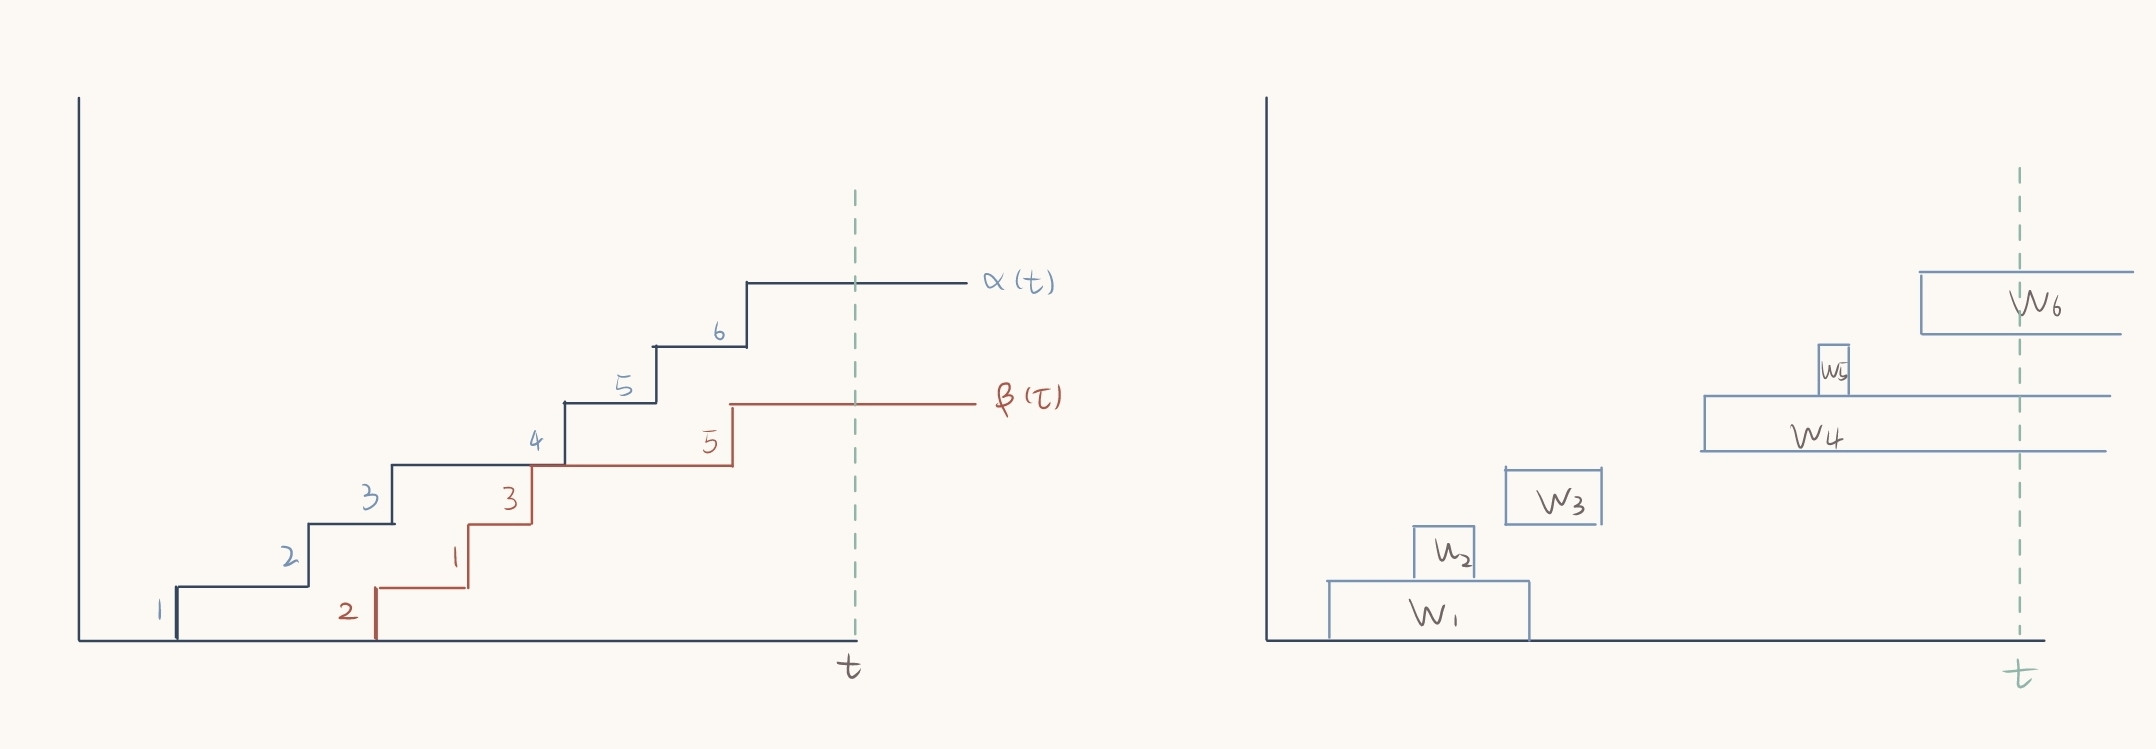
\includegraphics[width=\textwidth]{document/4-1.jpg}
\end{figure}

\section{The exponential distribution}
Recall that in a Markovian queueing system. $A/B/s$ both $A=M$(interarrival time) and $B = M$(service time) follow the exponential distributions, with DF and PDF of the form

\begin{align*}
    F(t) &= \mathbb{P}(T\leqslant t) = \left\lbrace\begin{array}{ll}
        1 - e^{-\gamma t} &\ \text{if}\ t\geqslant 0 \\
        0 & \ \text{if} \ t<0
    \end{array} \right. \\
    f(t) & = \left\lbrace\begin{array}{ll}
        \gamma e^{-\gamma t} &\ \text{if}\ t\geqslant 0 \\
        0 & \ \text{if} \ t<0
    \end{array} \right.
\end{align*}
for some $\gamma>0$, where $T$ is the $A$ or $B$ RV. We have 
\begin{align*}
    \mathbb{E} T &= \int_0^{\infty} \gamma u e^{-\gamma u} du = \frac{1}{\gamma} \\
    \text{var} T &= \mathbb{E}(T^2) - (\mathbb{E} T)^2 = \int_0^{\infty} \gamma u^2 e^{-\gamma u} du - \frac{1}{\gamma^2} = \frac{1}{\gamma^2}
\end{align*}

\setcounter{proposition}{1}
\begin{proposition}
    $f(t)$ is strictly decreasing for $t\geqslant 0$. Thus, 
    \begin{align*}
        \mathbb{P}(0\leqslant T\leqslant h) > \mathbb{P}(t\leqslant T\leqslant t+h),\quad \forall t,h >0
    \end{align*}
    \begin{figure}[H]
        \centering
        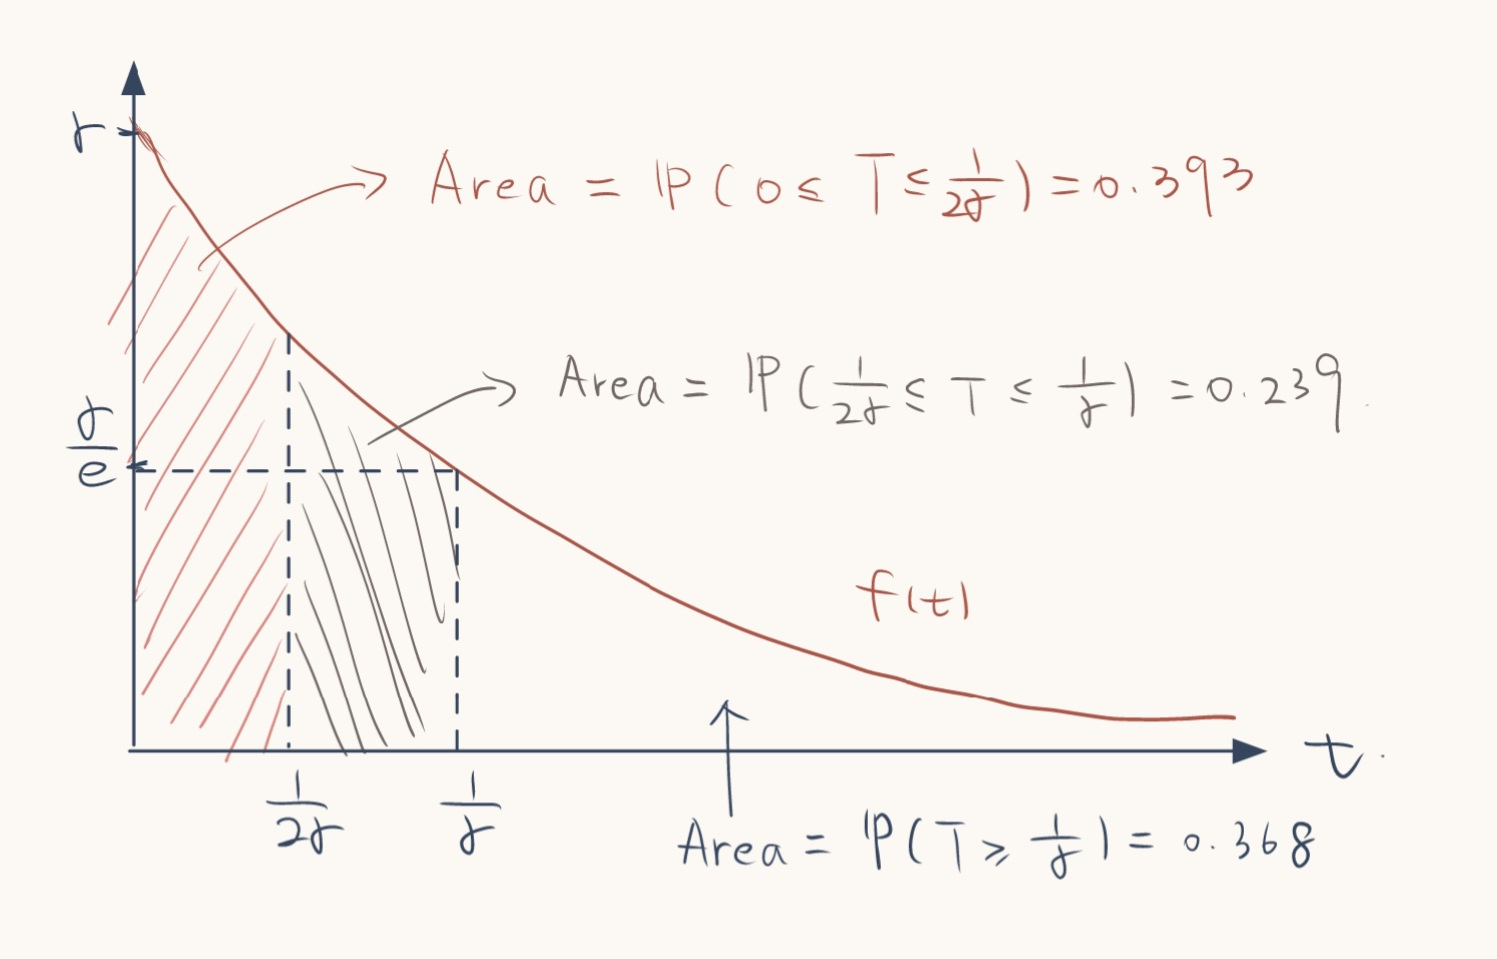
\includegraphics[width = 0.6\textwidth]{document/4-2.jpg}
    \end{figure}
\end{proposition}

\paragraph{Recall} For events $E_1,E_2$ in a probability space, the \uline{conditional probability} of $E_1$, gives $E_2$, is
\begin{align*}
    \mathbb{P}(E_1\mid E_2) = \frac{\mathbb{P}(E_1\cap E_2)}{\mathbb{P}(E_2)}
\end{align*}

\begin{proposition}[Lack of memory]
    \begin{align*}
        \mathbb{P}(T>t+h\mid T>h) = \mathbb{P}(T>t) \quad \forall t,h>0
    \end{align*}
    That is, the probability distribution of the remaining time until the event (arrival or service completion) occurs is always the same, regardless of how much time $h$ has already passed. There is no memory of what has already occurred.
\end{proposition}
\begin{proof}
    \begin{align*}
        \mathbb{P}(T>t+h\mid T>h) &= \frac{\mathbb{P}(T>t+h\ \text{and}\ T>h)}{\mathbb{P}(T>h)} = \frac{\mathbb{P}(T>t+h)}{\mathbb{P}(T>h)} \\
        &= \frac{e^{-\gamma (t+h)}}{e^{-\gamma h}} = e^{-\gamma t} = \mathbb{P}(T>t)
    \end{align*}
\end{proof}

\begin{proposition}
    Let $T_1,\cdots,T_n$ be independent exponential RVs with parameters $\gamma_1,\cdots,\gamma_n$. Then the RV 
    \begin{align*}
        U = \min(T_1,\cdots, T_n)
    \end{align*}
    has an exponential distribution with parameter $\gamma = \gamma_1 + \cdots + \gamma_n$. Thus, if $T_i$ represents the time until the $i^{\text{th}}$ event occurs, then $U$ represents the time until the first of the $n$ events occurring. 
\end{proposition}
\begin{proof}
    \begin{align*}
        \mathbb{P}(U>t) &= \mathbb{P}(T_1>t,\cdots, T_n>t\ \text{all hold}) \\
        & = \eqnmarkbox[blue]{1}{\mathbb{P}(T_1>t) \cdots \mathbb{P}(T_n>t)} \\
        & = e^{-\gamma_1 t} \cdots e^{-\gamma_n t} = e^{-\gamma t}
    \end{align*}
    \annotate[yshift=2.5em]{above,right}{1}{By independence}
    
\end{proof}

In particular, if $X_1,\cdots,X)s$ are the independence service times, each exponential with parameter $\mu$, then $U$ is the time until the next service completion, which is the exponential with parameter $s\mu$.

\subsubsection{Relationship with Poisson distribution and process}
Suppose the time between consecutive occurrences of some kind of event (For example, interarrivals) has an exponential distribution with parameter $\gamma$. Let $Y(t)$ be the number of event occurrences at time $t\geqslant 0$. Then $Y(t)$ is a RV with the Poisson Distribution with parameters $\gamma t$, given by
\begin{align*}
    \mathbb{P}(Y(t) = k) = \frac{(\gamma t)^k e^{-\gamma t}}{k!},\quad  \text{for}\ k=0,1,2,\cdots
\end{align*}
When the events are counted on a continuing basis, the counting process $\{Y(t):t\geqslant 0\}$ is a \uline{Poisson process} with mean rate $\gamma$.

\begin{proposition}
    \begin{align*}
        \mathbb{P}(T\leqslant t+h\mid T>t) \approx \gamma h,\quad \forall t>0\ \text{and small}\ h
    \end{align*}
\end{proposition}
\begin{proof}
    \begin{align*}
        \mathbb{P}(T\leqslant t+h\mid T>t) &= \frac{\mathbb{P}(T\leqslant t+h\ \text{and}\ T>t)}{\mathbb{P}(T>t)} \\
        &= \frac{(1-e^{-\gamma(t+h)}) - (1-e^{-\gamma t})}{e^{-\gamma t}} \\
        &= 1 - e^{-\gamma h} \approx \gamma h \ \text{for small}\ h
    \end{align*}
\end{proof}

Note that Prop 4.3 says that the probability of an event occurring within an interval of fixed length $h$ is constant, regardless of how much time has passed. Prop 4.5 says that if $h$ is small, then this constant probability is approximately $\gamma h$.


\section{Birth-Death Process and M/M/s Systems}
Recall that $\mathbb{P}_k(t) = $ Probability that state $=k\geqslant 0$ at time $t\geqslant 0$ in a queueing system.
\begin{definition}
    A queueing system is in \uline{transient state} if $\mathbb{P}_k(t)$ depends on $t$. The system becomes \uline{steady state} if $\mathbb{P}_k(t)$ becomes independent of $t$ if $t\geqslant t_1$ for some (large) time $t_1$. If the system is in steady state, let
    \begin{align*}
        p_k = \text{Probability that state} = k \geqslant 0
    \end{align*}
    The \uline{birth-death process} describe the state of a queueing system over time. If the system is Markovian, we assume the following:
    \begin{itemize}
        \item[(1)] Given $N(t) = k$, the probability distributions of the remaining times until the next ``birth'' (arrival) and next ``death'' (departure) are exponential with parameters $\lambda_k,\mu_k$.
        \item[(2)] All RVs in (1) are mutually independent. The next change in state is 
        
        \begin{center}
            \begin{tabular}{lll}
            either: & $k\to k+1$ & (a birth) \\
            or: & $k\to k-1$ & (a death)
        \end{tabular}
        \end{center}     
    \end{itemize}
\end{definition}

\begin{remark}
    By Prop 4.3, for the Markovian birth-death process, the future depends only on the current state, and is independent of any past events. The process is thus a \text{continuous time Markov chain}.
\end{remark}

The relation of the exponential distribution to the Poisson process implies that the $\lambda_k$ and $\mu_k$ are mean rates.

Assume that a queueing system can reach steady state. Let $u_k(t)$ and $v_k(t)$ be the number of times the birth-death process enters and leave state $k$ in $[0,t]$. Then $|u_k(t) - v_k(t)| \leqslant 1$, so
\begin{align*}
    \lim\limits_{t\to\infty} \left|\frac{u_k(t)}{t} - \frac{v_k(t)}{t}\right| = 0
\end{align*}

Since $\frac{u_k(t)}{t}$ and $\frac{v_k(t)}{t}$ are the mean rates at which the process enters and leaves state $k$, we have:
\begin{proposition}[Rate in $=$ Rate out Principle]
    For any state $k\geqslant 0$ in a Markovian birth-death Process, 
    \begin{align}
        \text{Mean entering rate}=\text{Mean leaving rate} \label{4.5}
    \end{align}

    An equation of the form \ref{4.5} is a \uline{balance equation}.
\end{proposition}

For state $0$, the process may only enter from state 1. In steady state, since $p_1$ is the proportion of time that the process can enter state $0$, the mean entering rate to state $0$ is $\mu_1 p_1$. Similarly, the mean leaving rate from state $0$ is $\lambda_0 p_0$. Thus \ref{4.5}$\Rightarrow$
\begin{align}
    \mu_1 p_1 = \lambda_0 p_0 \label{4.6}
\end{align}

For any other state $k\geqslant 1$, we similarly have 
\begin{align}
    \lambda_{k-1}p_{k-1} + \mu_{k+1}p_{k+1} = (\lambda_k + \mu_k) p_k \label{4.7}
\end{align}
Now, \ref{4.6} $\Rightarrow\ \mu_1 p_1 - \lambda_0 p_0 = 0$. And \ref{4.7} $= \mu_{k+1}p_{k+1} - \lambda_k p_k = \mu_k p_k - \lambda_{k-1}p_{k-1}$, $\forall k\geqslant 1$. Thus $\mu_k p_k - \lambda_{k-1}p_{k-1} = 0$, $\forall k\geqslant 0$.

We have
\begin{align*}
    p_k &= \frac{\lambda_{k-1}}{\mu_k} p_{k-1} + \frac{1}{\mu_k} \left(\mu_{k-1}p_{k-1} - \lambda_{k-2}p_{k-2} \right) = \frac{\lambda_{k-1}}{\mu_k} p_{k-1}  \\
    &= \cdots = \frac{\lambda_{k-1}\lambda_{k-2}\cdots \lambda_0}{\mu_k \mu_{k-1}\cdots \mu_0} p_0
\end{align*}

Let
\begin{align}
    r_k = \frac{\lambda_{k-1}\lambda_{k-2}\cdots\lambda_0}{\mu_k\mu_{k-1}\cdots \mu_0},\ \forall k\geqslant 1,\quad \text{and}\ r_0 = 1 \label{4.8}
\end{align}

Then $p_k = r_kp_0$, $\forall k\geqslant 0$. Since $\sum\limits_{k=0}^{\infty} p_k = 1$, we have
\begin{align}
    p_0 = \left( \sum\limits_{k=0}^{\infty} r_k\right)^{-1} \label{4.9}
\end{align}

We remark that steady state cannot be reached if $\lambda_k,\mu_k$ are s.t. $\sum\limits_{k=0}^{\infty} r_k = \infty$. If $\lambda,\mu$ and $\rho = \frac{\lambda}{s\mu}$ are as in section 4.1, then steady state can be reached if $\rho < 1$.

If $s$, $\overline{L}$, $\overline{L}_q$ as defined in section 4.1, and $\overline{\lambda}$ is as in \ref{4.2}, then 
\begin{align}
    \overline{L} = \sum\limits_{k=0}^{\infty} kp_k,\quad \overline{L}_q = \sum\limits_{k=s}^{\infty} (k-s)p_k,\quad \text{and} \quad \overline{\lambda} = \sum\limits_{k=0}^{\infty} \lambda_k p_k \label{4.10}
\end{align}

Now, consider the M/M/1 system. For $\lambda, \mu,\rho$ as above, with $\rho = \frac{\lambda}{\mu} < 1$, we have

\ref{4.8} $\Rightarrow\ r_k = \left(\frac{\lambda}{\mu}\right)^k = \rho^k$, $\forall k\geqslant 0$.

\ref{4.9} $\Rightarrow\ p_o = \left(\sum\limits_{k=0}^{\infty} r_k\right)^{-1} = \left(\sum\limits_{k=0}^{\infty} \rho^k \right)^{-1} = 1 - \rho$.

\ref{4.10} $\Rightarrow\ \overline{L} = \sum\limits_{k=0}^{\infty} kp_k = \sum\limits_{k=0}^{\infty} kr_kp_0 = (1-\rho) \sum\limits_{k=0}^{\infty} k\rho^k = (1-\rho) \rho \frac{d}{d\rho}\sum\limits_{k=0}^{\infty} \rho^k = (1-\rho) \rho \frac{d}{d\rho} \frac{1}{1-\rho} = \frac{\rho}{1-\rho} = \frac{\lambda}{\mu - \lambda}$

Similarly, \ref{4.10} $\Rightarrow$
\begin{align*}
    \overline{L}_q &= \sum\limits_{k=1}^{\infty} (k-1)p_k = \overline{L} - (1-p_0) = \frac{\lambda^2}{\mu(\mu - \lambda)}
\end{align*}

Note that if $\rho = \frac{\lambda}{\mu} > 1$, then $\sum\limits_{k=0}^{\infty} r_k = \sum\limits_{k=0}^{\infty} \rho^k = \infty$, and we cannot have steady state.

Back to $\rho<1$. Let $W$ be a sojourn time RV. If the customer $C$ finds $k$ customers in the queue, then $C$ has to wait through $k + 1$ service times, including $C$'s own, but not the customer currently in service (see Prop 4.3). If $X_1,\cdots, X_{k+1}$ are the RVs of the service times, each exponential with parameter $\mu$, then letting $S_{k+1} = X_1 + \cdots + X_{k+1}$, $k\geqslant 0$, we have
\begin{align*}
    \mathbb{P}(W>t) = \sum\limits_{k=0}^{\infty} p_k \mathbb{P}(S_{k+1}>t)
\end{align*}

It can be shown from this that 
\begin{align*}
    \mathbb{P}(W>t) = e^{-\mu(1-\rho)t},\quad t\geqslant 0
\end{align*}

Thus, $W$ has the exponential distribution with parameter $\mu(1\rho)$, and 
\begin{align*}
    \mathbb{E} W = \frac{1}{\mu(1-\rho)} = \frac{1}{\mu - \lambda}
\end{align*}

Similarly, let $W_q$ be a queueing time RV. If $C$ finds no customers already in the system, then $\mathbb{P}(W_q = 0) = 1-\rho$. If $c$ finds $k\geqslant 1$ customers in the system, then $C$ has to wait through $k$ service times, so 
\begin{align*}
    \mathbb{P}(W_q > t) &= \sum\limits_{k=1}^{\infty} p_k \mathbb{P}(S_k>t) = \sum\limits_{k=1}^{\infty} (1-\rho)\rho^k \mathbb{P}(S_k>t) \\
    &= \rho\sum\limits_{k=0}^{\infty} p_k \mathbb{P}(S_{k+1}>t) = \rho\mathbb{P}(W>t) \\
    & = \rho e^{-\mu(1-\rho)t},\quad t\geqslant 0
\end{align*}

And $\mathbb{E} W_q = \mathbb{E} W - \frac{1}{\mu} = \frac{\lambda}{\mu(\mu - \lambda)}$.

We see that $W_q$ does not have an exponential distribution. But the conditional distribution 
\begin{align*}
    \mathbb{P}(W_q>t\mid W_q>0) = \frac{\mathbb{P}(W_q>t)}{\mathbb{P}(W_q>0)} = e^{-\mu(1-\rho)t},\quad t\geqslant 0
\end{align*}
is exponential with parameter $\mu(1-\rho)$.

Next, consider an M/M/s system $(s\geqslant 2)$. We can obtain (still $\lambda,\mu$ constants, and $\rho = \frac{\lambda}{s\mu}$)
\begin{align}
    r_k = \left\lbrace\begin{array}{ll}
        \frac{1}{k!}\left(\frac{\lambda}{\mu}\right)\eqnmarkbox[blue]{1}{^k},&\quad  1\leqslant k\leqslant s \\
        \frac{1}{s!}\left(\frac{\lambda}{\mu}\right)^s\rho^{k-s} = \frac{1}{s!s^{k-s}}\left(\frac{\lambda}{\mu}\right)^k& \quad k\geqslant s
    \end{array} \right.\label{4.11}
\end{align}

If $\rho = \frac{\lambda}{s\mu} <1$, then \ref{4.9}, \ref{4.11}$\Rightarrow$
\begin{align*}
    p_0 &= \left(\sum\limits_{k=0}^{\infty} r_k\right)^{-1} = \left(\sum\limits_{k=0}^{n-1} \frac{1}{k!}\left(\frac{\lambda}{\mu}\right)^k + \sum\limits_{k=s}^{\infty} \frac{1}{s!} \left(\frac{\lambda}{\mu}\right)^s \frac{1}{1-\rho} \right)^{-1} 
\end{align*}

Also, $p_k = r_k p_0$ for $k\geqslant 1$, where $r_k$ is as in \ref{4.11}, \ref{4.10}$\Rightarrow$
\begin{align*}
    \bar{L}_q = \frac{p_0 \rho}{s!(1-\rho)}\left(\frac{\lambda}{\mu}\right)^s
\end{align*}

and Th 4.1 (Little's Law), \ref{4.4}$\Rightarrow$
\begin{align*}
    \overline{W}_q = \frac{\overline{L}_q}{\lambda},\quad \overline{W} = \overline{W}_q + \frac{1}{\mu},\quad \overline{L} = \lambda \overline{W} = \lambda \overline{W} + \frac{\lambda}{\mu} = \overline{L}_q + \frac{\lambda}{\mu}
\end{align*}

We can also obtain:
\begin{align*}
    \mathbb{P}(W>t) &= e^{-\mu t} \left( 1 + \frac{p_0}{s!(1-\rho)} \left(\frac{\lambda}{\mu}\right)^s \dfrac{1 - e^{-\mu t(s - 1 - \frac{\lambda}{\mu})}}{ s - 1 - \frac{\lambda}{\mu}}\right) \\
    \mathbb{P}(W_q > t) &= (1-\mathbb{P}(W_q = 0))e^{-s\mu(1-\rho)t},
\end{align*}
where $\mathbb{P}(W_q = 0) = \sum\limits_{k=0}^{s-1} p_k$.

\setcounter{example}{2}
\begin{example}
    Suppose in a M/M/s system, a time unit is one hour. On average, a customer arrives every 30 minutes, and is served every 20 minutes. Then $\lambda = 2$ customers/hour, and $\mu = 3$ customers/hour. Since $\rho = \frac{2}{3s}<1$, the system is in steady state $\forall s\geqslant 1$. We have the following various values for $s = 1, 2$.
\end{example}

\begin{table}[H]
    \centering
    \begin{tabular}{|c|c|c|}
        \hline
         & $s=1$ & $s=2$ \\
         \hline
        $\rho$ & $\frac{2}{3}$ & $\frac{1}{3}$ \\
        $p_0$ &  $\frac{1}{3}$ & $\frac{1}{2}$ \\
        $p_1$ &  $\frac{2}{9}$ & $\frac{1}{3}$ \\
        $p_k$, $k\geqslant 2$ & $\frac{1}{3}\left(\frac{2}{3}\right)^k$ & $\left(\frac{1}{3}\right)^k$\\
        $\overline{L}_q$ & $\frac{4}{3}$ & $\frac{1}{12}$\\
        $\overline{L}$ & $2$ & $\frac{3}{4}$ \\
        $\overline{W}_q$ & $\frac{2}{3}$ hour & $\frac{1}{24}$ hour\\
        $\overline{W}$ & $1$ hour & $\frac{3}{8}$ hour \\
         \hline
    \end{tabular}
\end{table}

